\section{Forums}

The forums feature will be examined based on a framework to determine how well the implemented feature has achieved its intended purpose and its functionality.

The feature analysis includes three sections:

\begin{enumerate}
    \item \textbf{Functional Requirements} - does the forum component meet the functional requirements defined in the project approach?
    \item \textbf{Non-Functional Requirements} - does the forum component meet the non-functional requirements defined in the project approach?
    \item \textbf{Usability Tests} - what do potential users of the system think about the forums and how could it be improved?
\end{enumerate}

This section will also contain a reflection on how well milestones were met compared to the timelines set at the start of this project, as well as the challenges faced throughout this project.

\subsection{Functional Requirements}
The functional requirements of the forums are evaluated based on whether or not they were implemented in the system.
A requirement is considered complete if most or all of its acceptance criteria have been met.
The priority of the requirement has also been taken into consideration.
If a "Must Have" criteria has not been completed, then the requirement also cannot be considered completed.
Requirements and criteria marked as "Won't Have" are not considered in this evaluation.

Below is the list of functional requirements and their acceptance criteria, each marked with their status of completion.

\begin{enumerate}
    \item Users can view a list of forum posts (Completed)
\end{enumerate}
\begin{itemize}
    \setlength{\itemindent}{1.5em}
    \item Users can see all forum posts in a table (Completed)
    \item Users can see all pinned posts in a separate table (Completed)
\end{itemize}

\begin{enumerate}
    \setcounter{enumi}{1}
    \item Users can clearly see which posts have been read and actioned (Completed)
\end{enumerate}
\begin{itemize}
    \setlength{\itemindent}{1.5em}
    \item Users can easily find answered posts (Completed)
    \item Users can sort posts by number of replies or comments (Completed)
    \item Users can see which posts have been endorsed (Completed)
\end{itemize}

\begin{enumerate}
    \setcounter{enumi}{2}
    \item Users can add a post to the forum (Completed)
\end{enumerate}
\begin{itemize}
    \setlength{\itemindent}{1.5em}
    \item Users can add a post with a title and description (Completed)
    \item Users can format their post description (Completed)
    \item Users can optionally attach files (Partially Completed)
    \item Users can optionally attach tags (Completed)
    \item Users can optionally attach links (Completed)
\end{itemize}

\begin{enumerate}
    \setcounter{enumi}{3}
    \item Users are able to search for a forum post (Completed)
\end{enumerate}
\begin{itemize}
    \setlength{\itemindent}{1.5em}
    \item Users can search a post's description or title (Completed)
\end{itemize}

\begin{enumerate}
    \setcounter{enumi}{4}
    \item Users can filter through forum posts (Completed)
\end{enumerate}
\begin{itemize}
    \setlength{\itemindent}{1.5em}
    \item Users can filter forum posts using pre-defined tags (Completed)
    \item Users can filter posts by those linked to announcements (Completed)
    \item Users can filter posts by those that are answered (Completed)
    \item Users can filter posts by those that are unanswered (Completed)
    \item Users can filter posts by those that are endorsed (Completed)
\end{itemize}

\begin{enumerate}
    \setcounter{enumi}{5}
    \item Users are able to sort the forum posts (Completed)
\end{enumerate}
\begin{itemize}
    \setlength{\itemindent}{1.5em}
    \item Users can sort forum posts by different headings in the post table (Completed)
\end{itemize}

\begin{enumerate}
    \setcounter{enumi}{6}
    \item Users can view the individual post details for a chosen post (Completed)
\end{enumerate}
\begin{itemize}
    \setlength{\itemindent}{1.5em}
    \item Users can navigate to a post page for an individual post (Completed)
    \item Users can easily see the post title, description, tags, author and data created (Completed)
    \item Users can see all the responses to the post (Completed)
    \item Users can see all the comments on the post (Completed)
\end{itemize}

\begin{enumerate}
    \setcounter{enumi}{7}
    \item Users can share a forum post with others (Partially Completed)
\end{enumerate}
\begin{itemize}
    \setlength{\itemindent}{1.5em}
    \item Users can copy a link to a forum post (Completed)
    \item Users can directly share a forum post to other platforms (Not Completed)
\end{itemize}

\begin{enumerate}
    \setcounter{enumi}{8}
    \item Users can upvote a forum post (Completed)
\end{enumerate}
\begin{itemize}
    \setlength{\itemindent}{1.5em}
    \item Users can upvote a post on the forum overview page (Completed)
    \item Users can upvote a post on the forum post page (Completed)
    \item Users can see the number of upvotes a post has (Completed)
\end{itemize}

\begin{enumerate}
    \setcounter{enumi}{9}
    \item Users can edit their post (Completed)
\end{enumerate}
\begin{itemize}
    \setlength{\itemindent}{1.5em}
    \item Users can edit a post after it has been posted (Completed)
\end{itemize}

\begin{enumerate}
    \setcounter{enumi}{10}
    \item User can delete their post (Completed)
\end{enumerate}
\begin{itemize}
    \setlength{\itemindent}{1.5em}
    \item Users can delete a post after it has been posted (Completed)
\end{itemize}

\begin{enumerate}
    \setcounter{enumi}{11}
    \item Users can comment on a post (Completed)
\end{enumerate}
\begin{itemize}
    \setlength{\itemindent}{1.5em}
    \item Users can leave a comment on a forum post (Completed)
    \item Users can format their comment (Completed)
    \item Users can edit their comment after it has been posted (Completed)
    \item Users can delete their comment after it has been posted (Completed)
\end{itemize}

\begin{enumerate}
    \setcounter{enumi}{12}
    \item Staff can manage the tags for the topic group (Completed)
\end{enumerate}
\begin{itemize}
    \setlength{\itemindent}{1.5em}
    \item Staff can add new tags (Completed)
    \item Staff can remove tags (Completed)
    \item Staff are unable to create duplicate tags (Completed)
    \item Students are unable to create tags (Completed)
\end{itemize}

\begin{enumerate}
    \setcounter{enumi}{13}
    \item Staff are able to pin posts to the top of the forums (Completed)
\end{enumerate}
\begin{itemize}
    \setlength{\itemindent}{1.5em}
    \item Staff can pin posts to the top of the forums (Completed)
    \item Staff can unpin posts to the top of the forums (Completed)
    \item Staff are unable to pin and unpin posts (Completed)
\end{itemize}

\begin{enumerate}
    \setcounter{enumi}{14}
    \item Staff can reply to a forum post (Completed)
\end{enumerate}
\begin{itemize}
    \setlength{\itemindent}{1.5em}
    \item Users can leave a reply on a forum post (Completed)
    \item Users can format their reply (Completed)
    \item Users can edit their reply after it has been posted (Completed)
    \item Users can delete their reply after it has been posted (Completed)
\end{itemize}

\begin{enumerate}
    \setcounter{enumi}{15}
    \item Staff can endorse a post or comment (Completed)
\end{enumerate}
\begin{itemize}
    \setlength{\itemindent}{1.5em}
    \item Staff can endorse a post (Completed)
    \item Staff can unendorse a post (Completed)
    \item Staff can endorse a comment (Completed)
    \item Staff can unendorse a comment (Completed)
\end{itemize}

\begin{enumerate}
    \setcounter{enumi}{16}
    \item Staff can directly link or embed materials to the forum post (Partially Completed)
\end{enumerate}
\begin{itemize}
    \setlength{\itemindent}{1.5em}
    \item Staff can add a direct link to a reply (Completed)
    \item Staff can embed course materials in a reply (Not Completed)
\end{itemize}

In total, 15 out of the 17 functional requirements were completed.
The remaining two functional requirements were only partially completed.
Each of these functional requirements had one acceptance criteria that was not implemented however, both of these were lower priority tasks.
Overall, all of the high and mid priority requirements were implemented into the system.

Below is a list of incomplete requirements and acceptance criteria, and the reason behind why they were not completed.

\subsubsection{Users can share a forum post with others}

\textit{Users can directly share a forum post to other platforms (Could have)}

The original idea was that the share button on individual posts would provide users with various platforms, like Facebook Messenger and WhatsApp, in which they could select to send a direct link to the forum post to.
As this was a lower priority task, time constraints meant that it was unable to be completed on time.
Furthermore, since this functionality could be achieved by using the copy link to clipboard button that was built early in the implementation process and pasting the link to share it,
it was decided that the focus should be shifted to ensure higher priority tasks are completed instead.

\subsubsection{Staff can directly link or embed materials to the forum post}

\textit{Staff can embed course materials in a reply (Could have)}

The ability for staff to directly embed course materials into their reply to a forum post was a low priority feature that would've been nice to have.
This would've allowed staff to easily provide students who are asking for help with references and materials that could assist them.
Similar to the previous requirement, there was not enough time to build this feature and since staff already had the option to include a link to resources in their reply, this criteria was considered unnecessary.

\subsubsection{Users can add a post to the forum}

\textit{Users can optionally attach files (Should have)}

While this requirement has been marked complete, it is important to note that the current state of the forums only allows for images to be attached to posts.
This criteria has been marked as partially complete as ideally, documents and videos should be able to be attached as well.
This was unable to be done, however, due to time constraints and lack of knowledge in handling these file types.
However, since a user can still add a new post, and screenshots are the most popular type of attachment in forums, this overall requirement has been marked as completed.

\subsection{Non-functional Requirements}
This section contains an evaluation of how performant and accessible the forum component is.

Using Google Lighthouse, tests were run and the forum component was given a score out of 100 for performance and accessibility.
Google Lighthouse also produced a report with more details on ways in which the forums could be improved to produce a higher score.

\subsubsection{Performance}

\begin{figure}[h!]
    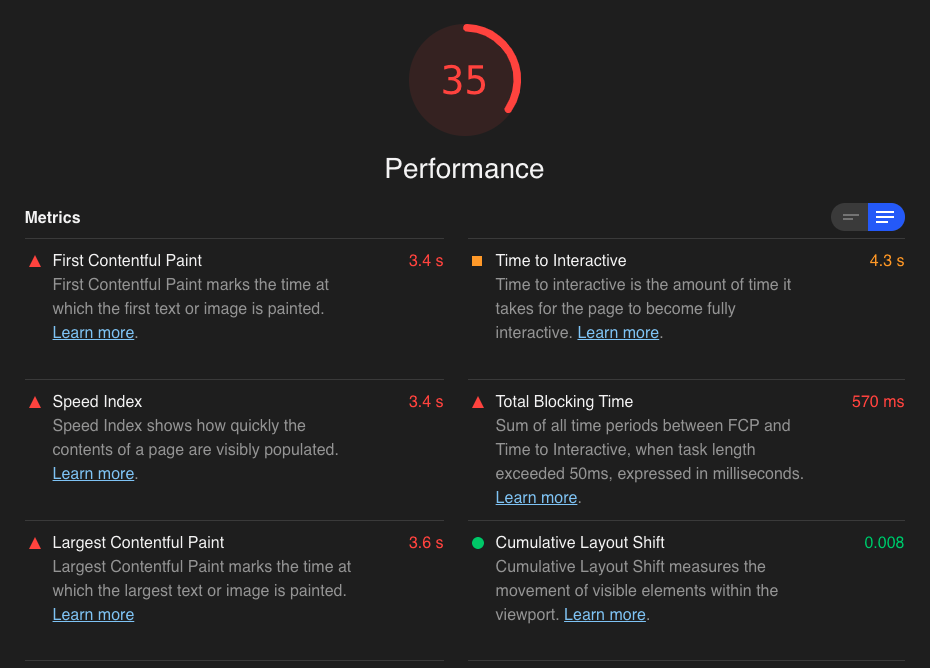
\includegraphics[scale=0.3]{forums-analysis-performance-overview-page.png}
    \centering
    \caption{Performance Report for Forums Overview Page}
\end{figure}

\begin{figure}[h!]
    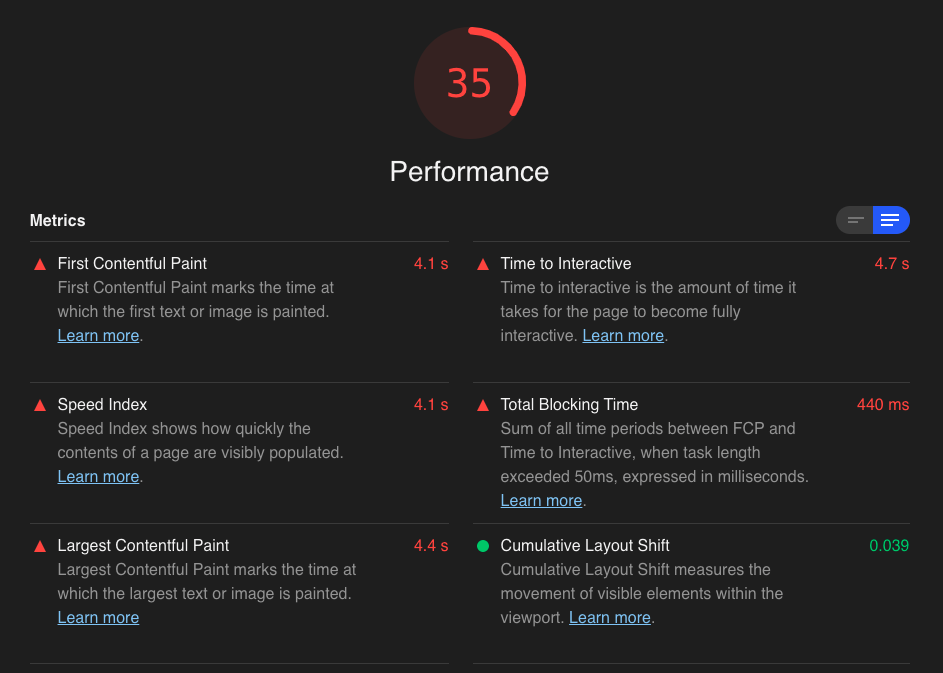
\includegraphics[scale=0.3]{forums-analysis-performance-post-page.png}
    \centering
    \caption{Performance Report for Forums Post Page}
\end{figure}

As seen from the figures above, the performance score for the forums are quite low, with a 35 out of 100 for both the overview and post pages.
Compared to the standards set by high-performing websites, the metrics measured show that the contents of the forum pages are slow to render and become interactive.
For a user with reasonable internet speeds, the slower renders would not be too noticeable.
The performance issues would mainly become a problem for users who have slow or throttled internet connections.
Despite this, performance is still an important factor when building a website and should definitely be improved in future iterations of the forum.
Refactoring the backend API and database to have a heavier focus on performance would be required to achieve this.
The report also suggests that reducing the amount of unused JavaScript could significantly reduce the load times.
This should definitely be addressed in future iterations.

On a positive note, the report shows that the forums pass the "Cumulative Layout Shift" metric.
This means that once the page has loaded, there is very minimal movement within the viewport of the user.
This is vital as it reduces the likelihood of misclicks for users.

\subsubsection{Accessibility}

\begin{figure}[h!]
    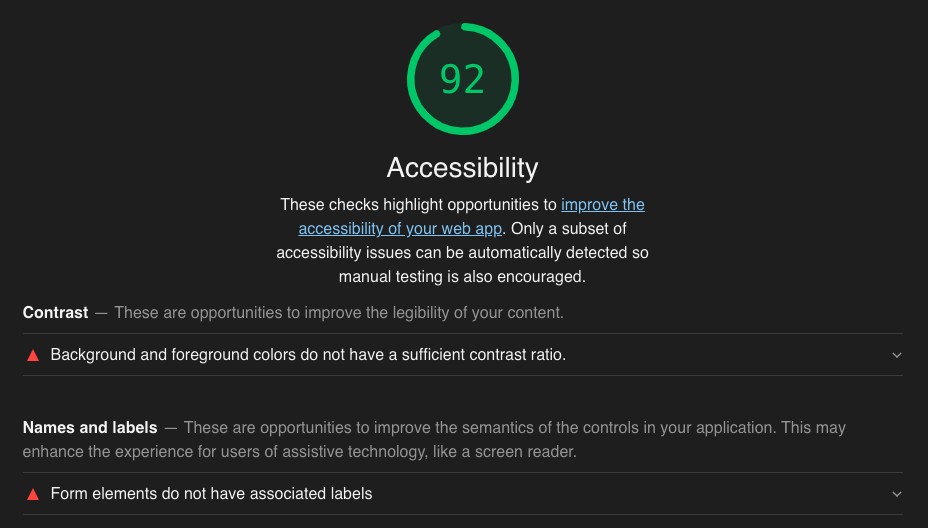
\includegraphics[scale=0.3]{forums-analysis-accessibility-overview-page.png}
    \centering
    \caption{Accessibility Report for Forums Overview Page}
\end{figure}

\begin{figure}[h!]
    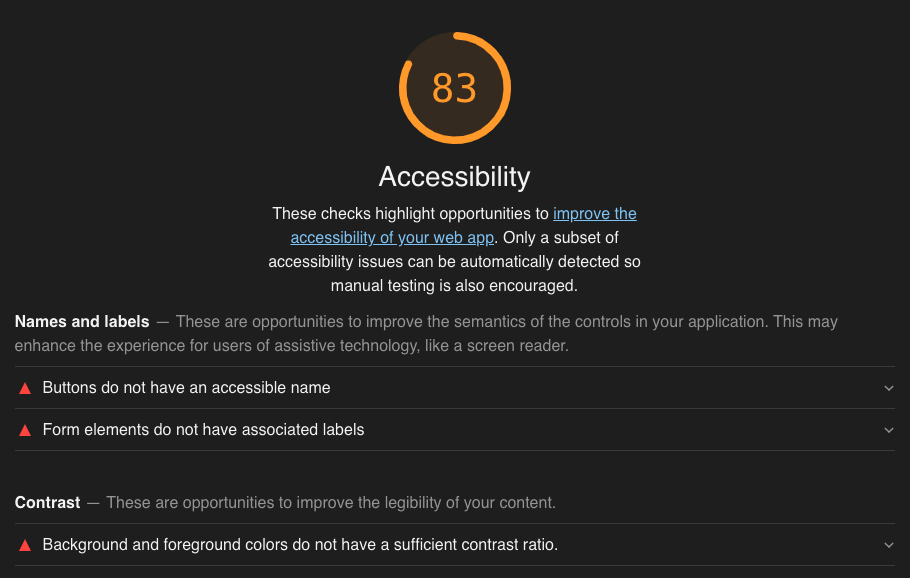
\includegraphics[scale=0.3]{forums-analysis-accessibility-post-page.png}
    \centering
    \caption{Accessibility Report for Forums Post Page}
\end{figure}

As seen from the figures above, the accessibility score for the forums was relatively high, with a 93 out of 100 for the overview page and a 83 out of 100 for the post pages.
A high accessibility score is essential for ensuring that all users, including those with disabilities, are able to use the system.
The score received for the forums is most likely due to the use of the Chakra-UI library which automatically applies a lot of the tags required for accessibility.
Even though these scores are quite high, the report suggests some easy improvements that can be made in future iterations to further improve the accessibility of the site.

Some of the colours used on both the overview and post pages do not have enough contrast with the background.
This means that people who are visually impaired may have trouble reading the words.
Since the background colour of the forums is white, making all the text darker on both pages would easily solve this problem.

A screenreader is a popular device for some people with disabilities as it can read out the components and text on a page.
As a result, it is important that all images, forms and buttons have alternative text that describes its purpose that can be read out by the device.
The report shows that on the post page, some of the buttons do not contain this alternative text.
In order to ensure that the button can be read out to users, an accessible name should be added to these buttons.
Labels should also be added to each of the input fields on the page, including those in the "Add Post" modal and in the responses and comments section of the post page.